\chapter{実装}
\label{chap:implementation}

% \section{めも}

% Linuxカーネルのバージョン,System.mapの情報およびconfigの情報を知らなければ,メモリのみから正しくコンテキストを復元していくことはできない.

% libtlpの論文(もうちょっとちゃんと書く)で紹介されているprocess-list.cはSystem.mapを引数として渡し,
% \verb|init_task|の行をreadすることでinit_taskの仮想アドレスを得ている.
% また,カーネルコンフィグに依存するマクロの値や,使用する関数などもハードコーディングされており,論文の環境以外で動かすことが容易ではない.

\section{実装の概要}

本研究では,RDMAを用いて,動作中のマシンのメモリの値を取得していくことで,リモートホストから監視対象ホストのオペレーティングシステムのコンテキストを復元していくことを目指す.
この目的を実現するために,本研究では,\cite{246316}を用いて実験を行う.

\section{nettlp}
\label{section:nettlp}

nettlp本来の目的は,PCIeデバイスの開発プラットフォームである.(リファレンス)

その機能の一つとして,DMA messageとethernetパケットを相互変換する機能がある.
\ref{chap:related_works}で述べたが,RDMAのInfiniband実装は,制限が多い.(もう少し詳しく)
nettlpにおけるRDMAでは,物理アドレスを指定することで,任意のバイト数(なんバイトだっけ?)の値を取得することが可能である.
また,アクセスできないメモリアドレスは存在しない,すなわち全メモリアドレス空間から値を取得することが可能となっている.

nettlpはFPGAボード上で動作するものであり,これを利用するためのインターフェースとして,libtlpが用意されている.
libtlpでは,RDMAを用いてメモリダンプを取得するためのインターフェースが関数として用意されている.
この関数を含んだヘッダファイルをincludeし,プログラムから呼び出すことで,メモリアドレスの値が返ってくる.

用意されている関数は,\verb|dma_read|関数と\verb|dma_write|関数の二つである.
\verb|dma_read|関数は,値を読みだすための関数であり,呼び出す際に読みたいメモリアドレスを渡す.
\verb|dma_write|関数は,値を指定した物理アドレスに書き込むための関数であり,呼び出す際に,書き込みたいメモリアドレスと値を渡す.

本研究では,\verb|dma_read|関数のみを用いる.

\subsection{process-list.c}

このファイルでやっていることをかく.
本研究の実装が,このprocess-list.cを拡張したものであるということを書く.

\section{実験環境}

本研究で実装を行う環境は,図\ref{fig:zentai}にあるように,nettlpが書き込まれたFPGAが刺さった監視対象ホストと,本研究における実装を実行するホストの2台で構成する.

監視対象ホストは,Linux 4.15.0-72-genericのubuntuであり,PCIeデバイスとして,nettlpが書き込まれたFPGAボードが刺さっている.
本研究では,FPGAボードとして,ザイリンクスのやつを使用している.
また,このFPGAボードは,ネットワークインターフェースでもあり,IPアドレスとして,192.168.10.1を静的に振ってある.

実装を実行するホストは,Linux 4.19.0-6-amd64のDebian busterであり,光ファイバーケーブル(名称はあとで修正)が刺さるNICを刺している.以後,実装ホストと呼称する.
このNICにはIPアドレスとして,192.168.10.3を静的に振ってある.
監視対象ホストに対してRDMAを実行する際は,\verb|dma_read|関数,あるいは\verb|dma_wirte|関数を通して192.168.10.1に対してIPパケットを送信している.

\begin{figure}[htbp]
    \caption{全体}
    \label{fig:zentai}
    \begin{center}
        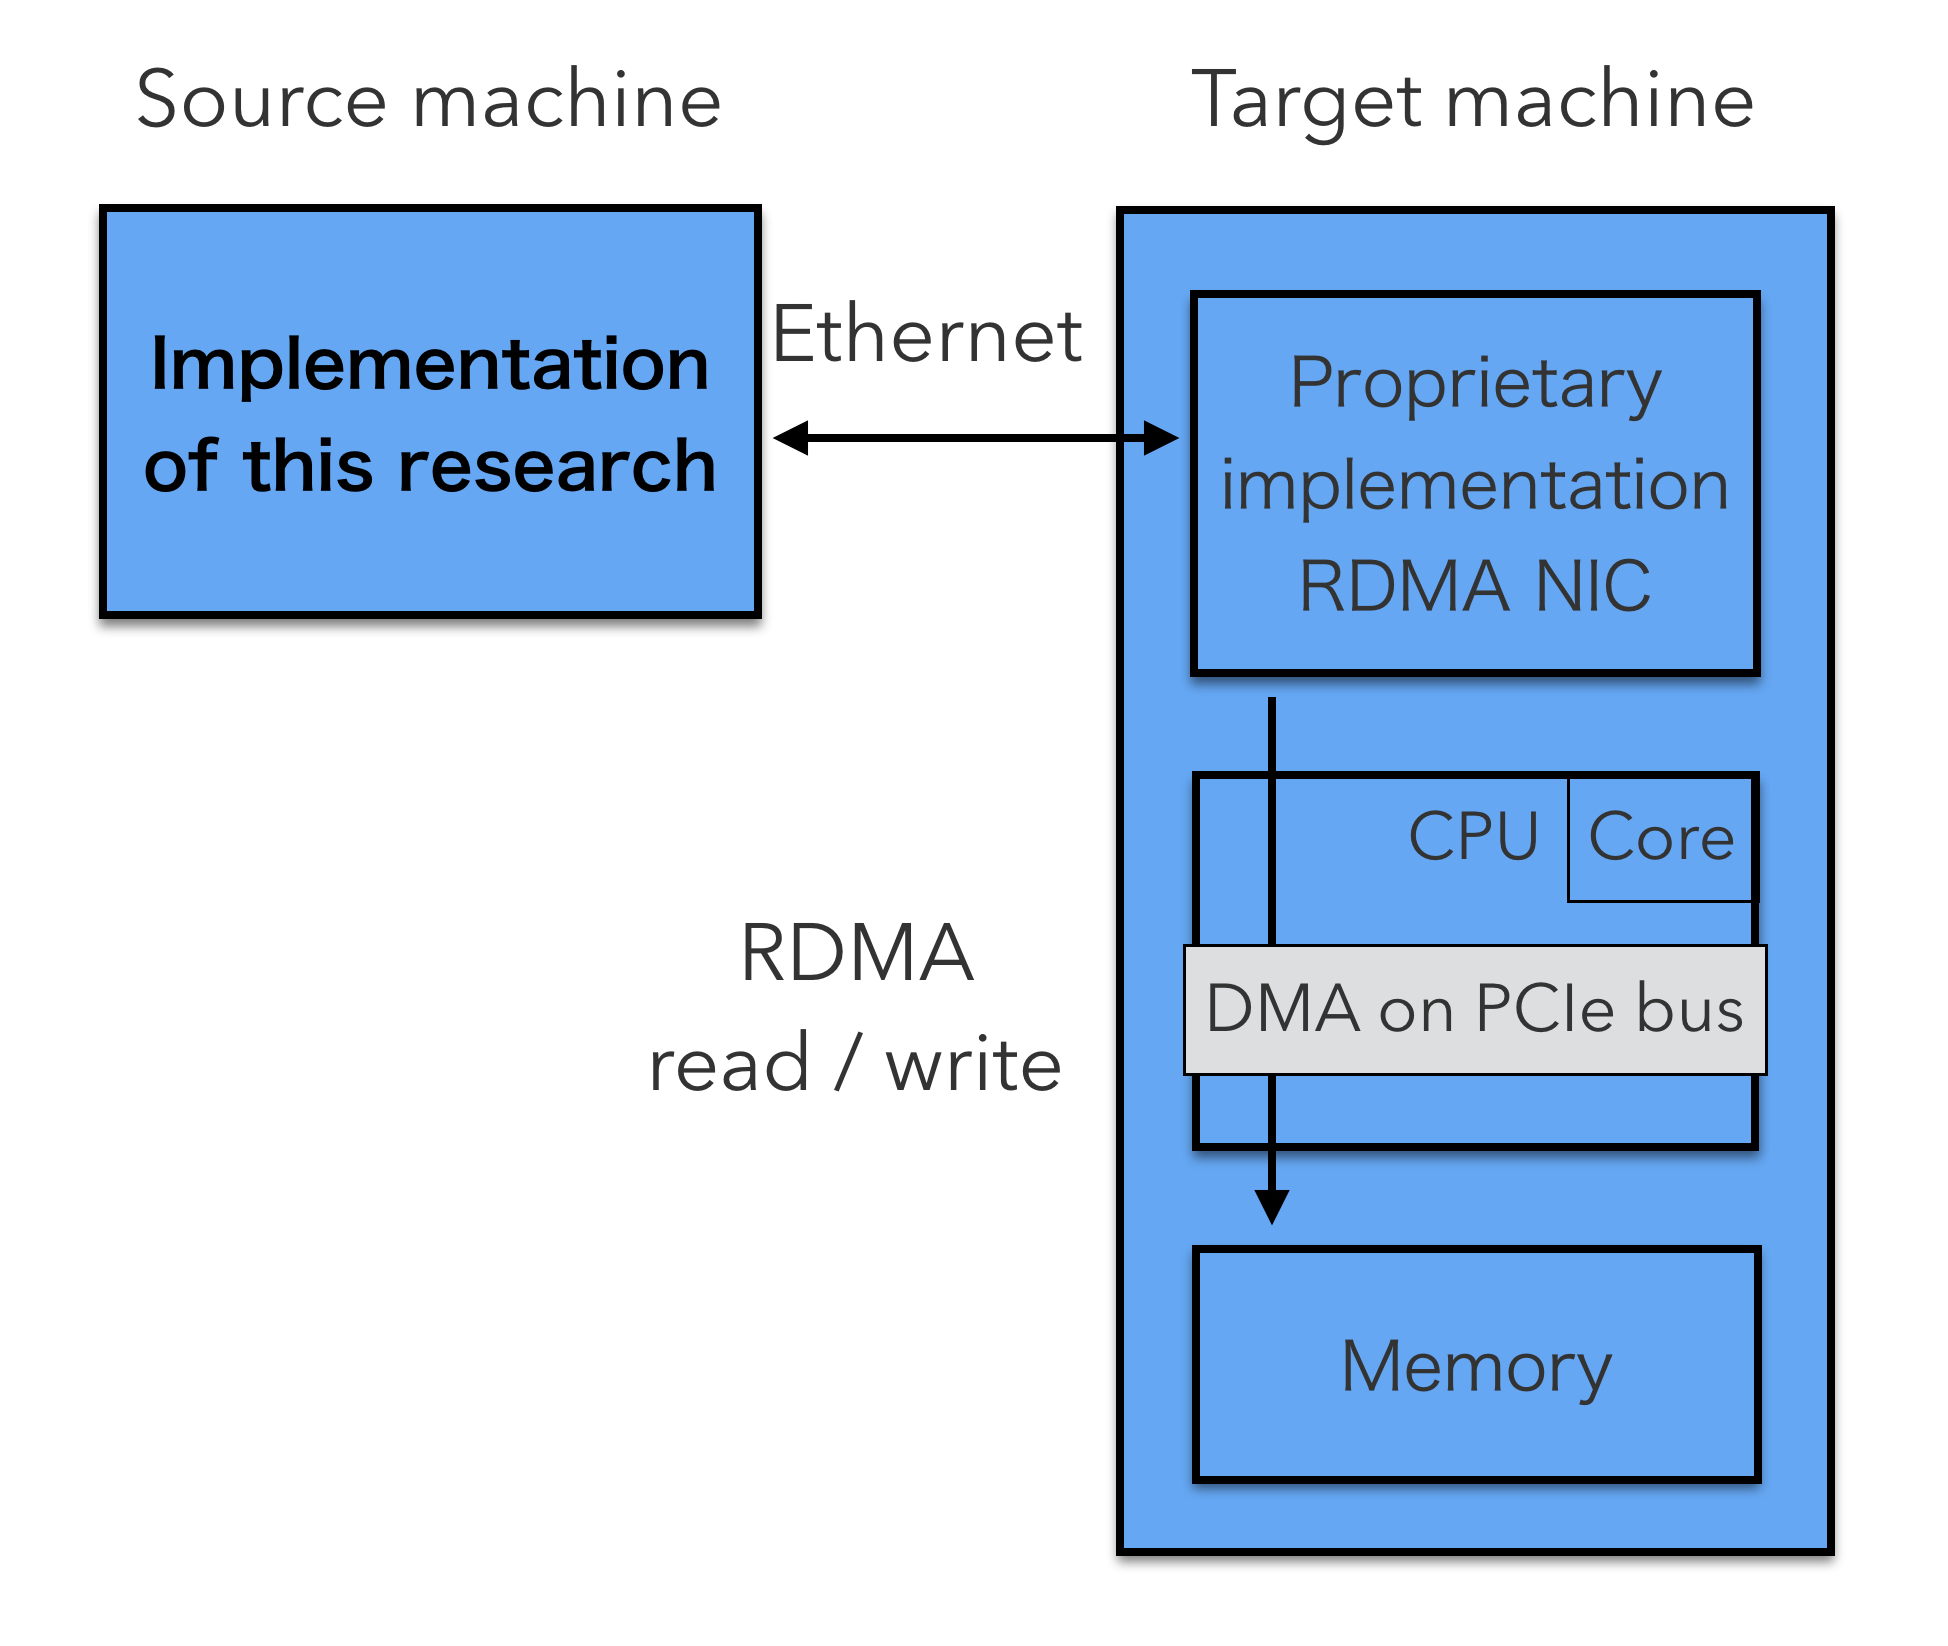
\includegraphics[bb=0 0 1000 800,width=15cm]{img/zentai.png}
    \end{center}
\end{figure}

\section{実装の前提情報}

本研究では,Linuxカーネルのバージョンは,実装ホストは知っている情報とする.
\label{section:want}で述べたもののうち,Linuxカーネルのバージョンだけは一旦Givenでやる.

また,KASLR(kernel address space layout randomization)を無効にしてある.

\subsection{KASLR}

KASLRの簡単な説明と,無効にする理由と無効にしても良い理由を書く.

\section{実装の全体}

ダンプしてくるということを書く.物理アドレスのマッピングに関しても

次の工程として,収集したカーネルコンフィグを元に手元のコンピュータでLinuxカーネルのソースコードに対してプリプロセスの処理を行い,task_struct型を確定する.
さらに,ソースコード上にある__phys_addrの実体を収集する.

最後に,この工程で得られた情報をもとに,libtlpで提唱されている手法を用いて,プロセスの一覧を正しく取得できることを確認する.

\section{工程1}

第一の工程として,RDMA NICを用いて,監視対象ホストのメモリを全探索し,メモリに落ちているSystem.mapのうち,init_taskが配置されている仮想アドレス空間に関する情報と,
Linuxカーネルにおける__phys_addr関数,task_struct型を決定するためのカーネルコンフィグに関する情報を収集することは\ref{chap:related_works}章で述べた.

(本セクションでは,その実装を詳しく書く.ダンプしまくるやつの説明をここに書く)

\section{工程2}

収集したカーネルコンフィグを元に手元のコンピュータでLinuxカーネルのソースコードに対してプリプロセスの処理を行い,task_struct型を確定する.
さらに,ソースコード上にある__phys_addrの実体を収集する部分に関する実装をより詳しく書く.

\section{工程3}

最後に,集められたデータをもとに,process-listを改造したものに関する説明をここに書く
